\clearpage
\subsection{Linked List} % (fold)
\label{sub:linked_list}

Pointers and dynamic memory allocation make it possible to store values in new and interesting ways. One way of structuring this data is to dynamically allocate each value, and link these together using pointers. An illustration of this is shown in \fref{fig:linked-list}.

Linked lists have the advantage of being very fast to perform insert and delete actions, when compared with arrays. The disadvantage is an increase in storage size to keep all the pointers, and the fact you must loop through the nodes to access any value in the list. 

\begin{figure}[htbp]
   \centering
   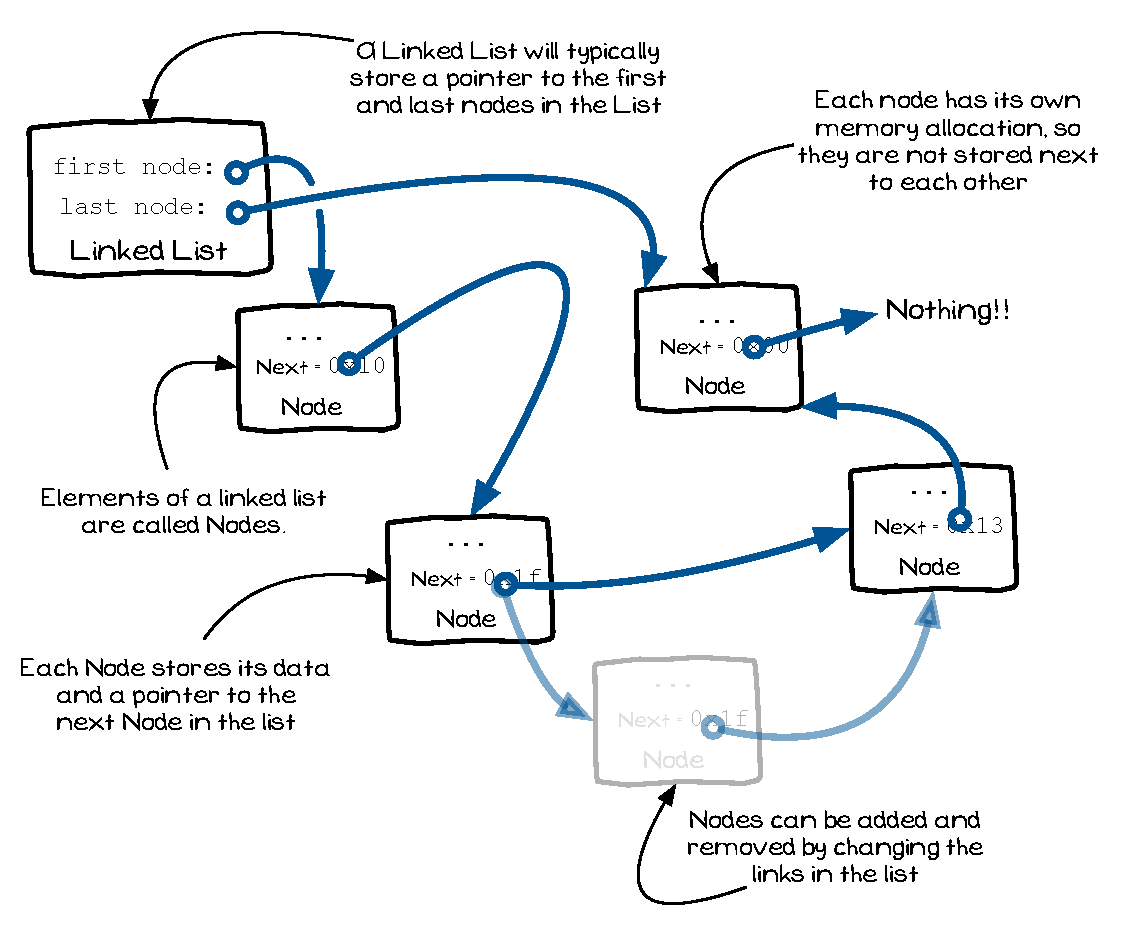
\includegraphics[width=0.90\textwidth]{./topics/dynamic-memory/diagrams/LinkedList} 
   \caption{Illustration of a linked list in memory}
   \label{fig:linked-list}
\end{figure}

\pseudocode{lst:iterate-linked-list}{Pseudocode for looping through a linked list}{topics/dynamic-memory/concepts/list-iterate.txt}

\mynote{
\begin{itemize}
  \item A Linked List is a \textbf{term} given to a certain way data can be structured in memory.
  \item A Linked List has \textbf{Nodes}, the equivalent of the elements of an array.
  \item Each \textbf{Node}, has some data and a pointer to the \textbf{Next} element in the list.
  \item The \textbf{Last} element in the list has \textbf{Nothing} as its next node.
  \item To access a Node in the list you must loop through from the first node until you reach the node you are after.
  \item You can insert and delete elements by changing the links in the list.
  \item If the grey node in \fref{fig:linked-list} is being \emph{inserted} then the previous node must be adjusted to point to it, and it to point to the next element of the list.
  \item If the grey node in \fref{fig:linked-list} is being \emph{deleted} then the previous node changes its link to skip that node and point to the next node in the list.
  \item The pseudocode in \lref{lst:iterate-linked-list} shows the standard way of applying an action to each node of a Linked List.
\end{itemize}
}

% subsection linked_list (end)